\documentclass[12pt]{article}

\usepackage[margin=1in]{geometry}
\usepackage{amsmath}
\usepackage{amsfonts}
\usepackage{amssymb}
\usepackage{amsthm}
\usepackage{mathtools}
\usepackage{mathrsfs}
\usepackage[ruled]{algorithm2e}

\newcommand\prn[1]{\left( #1 \right)}
\newcommand\bkt[1]{\left[ #1 \right]}
\newcommand\set[1]{\left\{ #1 \right\}}
\newcommand\abs[1]{\left| #1 \right|}
\renewcommand\epsilon{\varepsilon}
\newcommand\RR{\mathbb{R}}
\newcommand\yy{\boldsymbol{y}}
\newcommand\YY{{\boldsymbol{Y}}}
\newcommand\YYY{\mathcal{Y}}
\newcommand\HH{\mathcal{H}}
\newcommand\rf{{\mathrm{rf}}}
\newcommand\te{{\mathrm{te}}}

\title{Detecting Change Points Using Kernel SVMs}
\author{Cody Buntain}
\date{}

\begin{document}

\maketitle

\section{Overview}

Offline, parametric methods for change point detection often outperform their online, non-parametric competitors, but the flexibility gained by looser model restrictions and the ability to run in a streaming context are at times more valuable.
The kernel-based change detection (KCD) algorithm proposed by Desbory et al. is one such online algorithm \cite{1468491}.
Rather than rely on a priori knowledge of the generating distribution for a given series of data, KCD instead leverages support vector machines (SVMs) to construct descriptions of the data in a higher dimensional space defined by some given kernel (for our cases, the radial basis function, or RBF, kernel).
One can then use these high-dimensional descriptions to develop a dissimilarity statistic that characterizes the differences in center and spread of two possible regimes in the data.
Additionally, SVM's popular kernel trick allows one to generate this dissimilarity statistic in input space rather than feature space.

\subsection{Geometric Interpretation}

Desobry et al. provide a compelling geometric interpretation of the KCD based on angles between vectors as a measure of dissimilarity and spread (see Figure \ref{fig:kcdGeo} for a two-dimensional view). 
This geometric interpretation exists in feature space and assumes that two one-class SVMs were used to describe data from a possible past regime and a possible future regime respectively. 
The angle between the vectors normal to the decision planes $\widehat{c_pc_f}$ can then be used as a dissimilarity metric between the two sets of data.
To account for within-class spread, the authors then normalize this angle by the sum of the angles between the respective normal vectors a support vector of each regime $\widehat{c_ps_p}$ and $\widehat{c_fs_f}$.
The result is the KCD dissimilarity statistic shown in Eq. \ref{eq:kcd}.

\begin{figure}[htbp]
\begin{center}
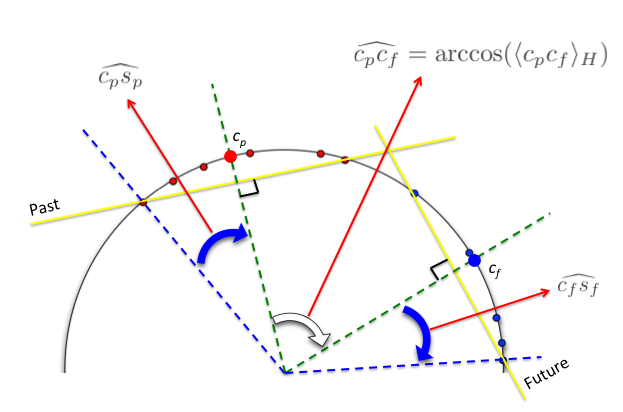
\includegraphics[width=0.667\textwidth]{kcd.png}
\caption{KCD Geometry in Feature Space}
\label{fig:kcdGeo}
\end{center}
\end{figure}

\begin{equation}
\label{eq:kcd}
KCD_{stat} = \frac{\widehat{c_pc_f}}{\widehat{c_fs_f} + \widehat{c_ps_p}}
\end{equation}

These angles can be calculated using the inverse cosine of the dot product between the weight vectors, as shown in Eq. \ref{eq:kcd2}.
One should note the denominator in Eq. \ref{eq:kcd2} is for normalizing the vectors to unit length.
This normalized dot product can be calculated in input space using SVM's learned weights $\boldsymbol{\alpha_p}$ and $\boldsymbol{\alpha_f}$ and the kernel matrices $K$ as shown in Eq. \ref{eq:kcd3}.
To obtain the within-class spread for each class, we use a similar form but rely on the SVM's intercept $\rho$ rather than a dot product, as shown in Eq. \ref{eq:kcd4}.

\begin{equation}
\label{eq:kcd2}
\widehat{c_pc_f} = \arccos \left(\frac{\langle w_p, w_f \rangle_F}{\| w_p \|\| w_f \|} \right)
\end{equation}

\begin{equation}
\label{eq:kcd3}
\frac{\langle w_p, w_f \rangle_F}{\| w_p \|\| w_f \|}  = \frac{\boldsymbol{\alpha}_p^T K_{p, f} \boldsymbol{\alpha}_f }{\sqrt{\boldsymbol{\alpha}_p^T K_{p, p} \boldsymbol{\alpha}_p }\sqrt{\boldsymbol{\alpha}_f^T K_{f, f} \boldsymbol{\alpha}_f }}
\end{equation}

\begin{equation}
\label{eq:kcd4}
\widehat{c_is_i} = \arccos \left(\frac{\rho_i}{\sqrt{\boldsymbol{\alpha}_i^T K_{i,i} \boldsymbol{\alpha}_i }} \right), i \in \{ p, f \}
\end{equation}

\section{Algorithm}

KCD has four parameters: 

\begin{itemize}
\item $m$ -- Window size, or the number of points on either side of a candidate change point.
\item $\gamma$ -- SVM parameter governing bandwidth for the RBF kernel (other kernels are possible, but we did not experiment with them).
\item $\nu$ -- One-class SVM parameter governing proportion of points that should be counted as outliers when training.
\item $\eta$ -- Threshold parameter such that, if $KCD_{stat} \ge \eta$ for some time point $h$, $h$ is considered a change point.
\end{itemize}

We assume $X$ is the input data of size $n \times k$.

\begin{function}[H]
	\SetAlgoLined
	$n \gets$ len$(X)$ \;
	\BlankLine
	changePoints $\gets [ \; ]$ \;
	\For{$h \in [m, n-m-1]$}{
		$X_{p} \gets X[h-m, h]$ \;
		$X_{f} \gets X[h, h+m]$ \;
		\BlankLine
		svm$_p \gets$ SVM.fit($X_{p}, \gamma, \nu$) \;
		svm$_f \gets$ SVM.fit($X_{f}, \gamma, \nu$) \;
		\BlankLine
		$\boldsymbol{\alpha}_p \gets \text{svm}_p.\alpha$ \;
		$\boldsymbol{\alpha}_f \gets \text{svm}_f.\alpha$ \;
		\BlankLine
		$\boldsymbol{\rho}_p \gets \text{svm}_p.\rho$ \;
		$\boldsymbol{\rho}_f \gets \text{svm}_f.\rho$ \;
		\BlankLine
		$K_{p, p} \gets \text{rbf}(X_p, X_p)$ \;
		$K_{f, f} \gets \text{rbf}(X_f, X_f)$ \;
		$K_{p, f} \gets \text{rbf}(X_p, X_f)$ \;
		\BlankLine
		$\widehat{c_pc_f} \gets \arccos \left(  \frac{\boldsymbol{\alpha}_p^T K_{p, f} \boldsymbol{\alpha}_f }{\sqrt{\boldsymbol{\alpha}_p^T K_{p, p} \boldsymbol{\alpha}_p }\sqrt{\boldsymbol{\alpha}_f^T K_{f, f} \boldsymbol{\alpha}_f }} \right)$ \;
		$\widehat{c_ps_p} \gets \arccos \left(  \frac{ |\boldsymbol{\rho}_p|}{\sqrt{\boldsymbol{\alpha}_p^T K_{p, p} \boldsymbol{\alpha}_p }} \right)$ \;
		$\widehat{c_fs_f} \gets \arccos \left(  \frac{ |\boldsymbol{\rho}_f|}{\sqrt{\boldsymbol{\alpha}_f^T K_{f, f} \boldsymbol{\alpha}_f }} \right)$ \;
		\BlankLine
		$KCD_{stat} \gets \frac{c_pc_f}{c_ps_p + c_fs_f}$ \;
		\If{$KCD_{stat} > \eta$}{
			changePoints += $h$
		}
	}
	\BlankLine
	return changePoints
 \caption{KCD($X, m, \gamma, \nu, \eta$) Algorithm by Desobry et al.\cite{1468491}}
\end{function}

\bibliographystyle{abbrv}
\bibliography{sources}

\end{document}

